\documentclass{article}
\usepackage{framed}
\usepackage{color}
\usepackage{graphicx}
\usepackage[utf8]{inputenc}
%\usepackage[unicode=true]{hyperref}
\usepackage{amsmath}
\usepackage{tikz}
\usetikzlibrary{shapes,arrows,automata,calc}
\usepackage[unicode=true,plainpages=false,colorlinks,linkcolor=cyan,citecolor=cyan,urlcolor=cyan,hyperindex=false]{hyperref}
\usepackage{attachfile}

\newcommand{\Constraint}[1]{\textsc{#1}}
\newcommand{\Tuple}[1]{\langle#1\rangle}  % #1 = tuple elements
\def\constraint#1{\textsc{#1}}


\setlength{\parindent}{0pt}
\setlength{\parskip}{4pt plus 2pt minus 1pt}
\usepackage[margin=1.60in]{geometry}

\definecolor{GRACeFULblue}{rgb}{0.20,0.60,0.86}
\begin{document}
\begin{center}
\includegraphics[width=5cm]{GRACeFULlogo.png}

\textcolor{GRACeFULblue}{Global systems Rapid Assessment tools\\
through Constraint FUnctional Languages}

\vspace{1cm}

FETPROACT-1-2014 Grant Nº 640954

\end{center}

\begin{framed}
\begin{center}
\Large
Constraints Composition Ops Library\\[1ex]

D5.2\\[1ex]

\end{center}
\end{framed}

\vspace{1cm}

\noindent
\begin{tabular}{@{}ll@{}}
  Lead Participant:       & Armines (Nicolas Beldiceanu, Ekaterina Arafailova, R\'emi Douence)
\\Partners Contributing:  & UPC
\\Dissemination Level:    & PU
\\Document Version:       & Final
\\Date of Submission:     & 2016-09-30
\\Due Date of Delivery:   & 2016-09-30
\end{tabular}

\clearpage
\section{Reading this document}

All cyan links of this document can be clicked in order to access
to the corresponding page on the web. This allows to put things in context.

In order to get the files attached to this document,
you are advised to use \href{https://get.adobe.com/fr/reader/}{\bf \textsf{Adobe Reader}} since
we are using the \LaTeX\ package \textsf{attachfile}
and since many PDF viewers do not support
attachments.

The source code of the \href{http://www.minizinc.org/}{\bf MiniZinc}
implementation as well as the instructions for using it are provided
as attached files
in this document available by clicking on the {\bf paper clip} icons
located in Section~\ref{sec:minizinc}. The same files are publicly available at 
\url{https://github.com/GRACeFUL-project}.

\section{Introduction}

This report itself is not the deliverable,
but summarises the content of the deliverable,
which consists of:
\begin{enumerate}
\item
The research papers done for bridging the gap
between the definition of constraints as composition of operators and
the synthesis of the corresponding code for handling these constraints.
The composition process is based on composing transducers, feature operators
and aggregator operators.
\item
An implementation in \href{http://www.minizinc.org/}{\bf MiniZinc}
of these constraints based on this composition process.
\end{enumerate}
Figure~\ref{fig:compositional} illustrates the definition of constraints
as multiple layers of operators, where the name of a constraint corresponds
to the concatenation of the operators used for defining it.

\begin{figure}[!b]
\centering
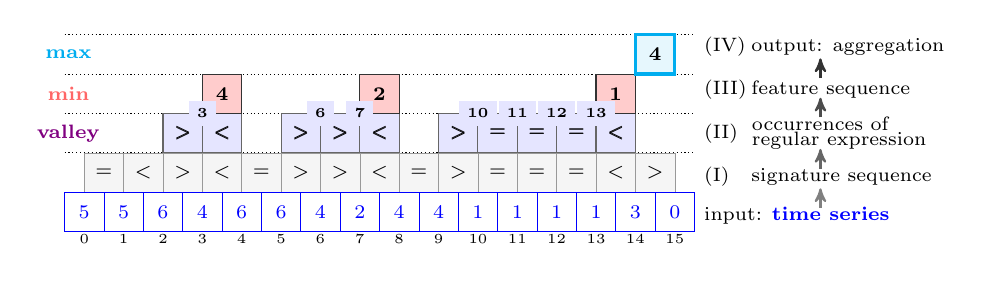
\begin{tikzpicture}
\begin{scope}[scale=0.5]
  \draw[thin,densely dotted] (0,5) -- (16,5); \draw[thin,densely
  dotted] (0,4) -- (16,4); \draw[thin,densely dotted] (0,3) --
  (16,3); \draw[thin,densely dotted] (0,2) -- (16,2);
  \node[font=\scriptsize] (min) at (0.1,4.5) {\color{cyan} \bf \constraint{max}};
  \node[font=\scriptsize] (min) at (0.1,3.5) {\color{red!60}\bf \constraint{min}};
  \node[font=\scriptsize] (min) at (0.1,2.5) {\color{violet}\bf \constraint{valley}};
  \draw[step=1cm,black!20,very thin,blue] (0,0) grid (16,1);
  \foreach[count=\i] \v in {0,...,15}
  \node[font=\tiny] (i\v) at (\i-0.5,-0.2) {\v};
  \foreach[count=\i] \v in {5,5,6,4,6,6,4,2,4,4,1,1,1,1,3,0}
  \node[font=\scriptsize] (v\v) at (\i-0.5,0.5) {\color{blue}\v};
  \foreach[count=\i] \c in {=,<,>,<,=,>,>,<,=,>,=,=,=,<,>} {
    \filldraw[fill=black!4,draw=black!40,very thin] (\i-0.5,1)
    rectangle (\i+0.5,2); \node[font=\scriptsize] (c\c) at (\i,1.5)
    {$\c$}; } \foreach \i/\p in
  {3/>,4/<,6/>,7/>,8/<,10/>,11/=,12/=,13/=,14/<} {
    \filldraw[fill=blue!10,draw=black!60,thin] (\i-0.5,2) rectangle
    (\i+0.5,3); \node[font=\scriptsize] (p\i) at (\i,2.5) {\color{black}$\mathbf{\p}$};
    \node[font=\scriptsize] (p\i) at (\i,2.52) {\color{black}$\mathbf{\p}$};}
  \foreach \i/\f in {8/2, 4/4,14/1} {
    \filldraw[fill=red!20,draw=black!80,thin] (\i-0.5,3) rectangle
    (\i+0.5,4); \node[font=\scriptsize] (f\i) at (\i,3.5)
    {\color{black}$\mathbf{\f}$}; }
  \filldraw[fill=cyan!10,draw=cyan,very thick] (15-0.5,4) rectangle
  (15+0.5,5); \node[font=\scriptsize] (a1) at (15,4.5)
  {$\mathbf{4}$}; \foreach \v/\i in
  {3/4,6/7,7/8,10/11,11/12,12/13,13/14}
  \node[font=\tiny] ( v\v) at (\i-0.5,3)
  {\colorbox{blue!10}{\color{black}\bf\v}}; \draw[very thin,blue] (0,1)
  -- (16,1); \node[anchor=west,font=\scriptsize] (level0) at
  (16,0.4-0.2+0.2) {input: {\color{blue}\bf time series}};
  \node[anchor=west,font=\scriptsize] (level1) at (16,1.4-0.2+0.2) {(I)};
  \node[anchor=west,font=\scriptsize] (level1) at (17.2,1.4-0.2+0.2)
  {signature sequence}; \node[anchor=west,font=\scriptsize] (level2)
  at (16,2.4+0.1) {(II)}; \node[anchor=west,font=\scriptsize] (level2) at
  (17.2-0.6,2.4+0.5-0.3+0.1-0.2) {\renewcommand{\arraystretch}{0.2}
    \begin{tabular}{l}occurrences of  \\ regular
                            expression \end{tabular}};
  \node[anchor=west,font=\scriptsize] (level2) at (17.2,2.4-0.3+0.2)
  {}; \node[anchor=west,font=\scriptsize] (level3)
  at (16,3.4+0.2) {(III)}; \node[anchor=west,font=\scriptsize]
  (level3) at (17.2,3.4+0.2) {feature sequence};
  \node[anchor=west,font=\scriptsize] (level3) at (16,4.7) {(IV)};
  \node[anchor=west,font=\scriptsize] (level3) at (17.2,4.7)
  {{\color{black}output}: aggregation};
  \draw[->,thick,black!50,>=stealth'] (19.2,0.6-0.2+0.2) -- (19.2,1.1-0.2+0.2);
  \draw[->,thick,black!60,>=stealth'] (19.2,1.6-0.2+0.2) -- (19.2,2.1-0.2+0.2);
  \draw[->,thick,black!70,>=stealth'] (19.2,2.6+0.3) -- (19.2,3.1+0.3);
  \draw[->,thick,black!80,>=stealth'] (19.2,3.6+0.3) -- (19.2,4.1+0.3);
\end{scope}
\end{tikzpicture}
\caption{Compositional constraint definition as multiple layers of operators: pattern, feature and aggregation operators
illustrating the constraint $\Constraint{\textcolor{cyan}{\bf max}\_\textcolor{red!60}{\bf
    min}\_\textcolor{violet}{\bf valley}} 
(\Tuple{5,5,6,4,6,6,4,2,4,4,1,1,1,1,3,0}, 4)$}
\label{fig:compositional}
\end{figure}

Attached to this document it provides an open implementation of these
constraints that uses the \href{http://www.minizinc.org/}{\bf MiniZinc}
modelling language as well as a quick start how to use this implementation
from existing solvers such as \href{http://www.choco-solver.org/}{\bf Choco}
or \href{https://sicstus.sics.se/}{\bf SICStus Prolog}.
The advantage of \href{http://www.minizinc.org/}{\bf MiniZinc} is to be interfaced
with many solvers both from Constraint Programming, SAT, MIP and local search.

\section{Summary of scientific publications}

The theory developed for synthesizing constraints from a functional specification is described in the following
three scientific publications.
\begin{enumerate}
\item
The way we describe constraints as a composition of operators and the way we synthesise
automata constraints from transducers are described in this first paper~\cite{CP15}.
The paper is freely accessible at \url{https://hal.inria.fr/hal-01370322}.
\item
The way we optimise the corresponding automata in a mechanical way is described in this second paper~\cite{CPAIOR16}.
The paper is freely accessible at \url{https://hal.inria.fr/hal-01355262}.
\item
Finally the way we come up with combinatorial objects that are parametrised by the operators used
in the constraint definition is described in this third paper~\cite{CP16}. These combinatorial objects
correspond to parametrised bounds and parametrised glue matrices that are used for synthesising
necessary conditions for the feasibility of each concrete constraint.
The paper is freely accessible at \url{https://hal.inria.fr/hal-01370317}.
\end{enumerate}
All three publications were presented at international conferences,
\href{http://booleconferences.ucc.ie/cp2015papers}{\bf CP~2015},
\href{https://symposia.cirrelt.ca/CPAIOR2016/en}{\bf CPAIOR~2016} and
\href{http://cp2016.a4cp.org/}{\bf CP~2016}. 

\section{MiniZinc implementation}\label{sec:minizinc}

\begin{itemize}
\item
A \href{http://www.minizinc.org/}{\bf MiniZinc} implementation of the time series constraints is available in this attached file
\attachfile[icon=Paperclip,mimetype=text/plain,description=time_series_constraints.mzn]{time_series_constraints.mzn}.
\item
Instructions how to use this \href{http://www.minizinc.org/}{\bf MiniZinc} implementation are given here
\attachfile[icon=Paperclip,mimetype=pdf/plain,description=Instructions.pdf]{Instructions.pdf}.
\item
Files referenced in the instructions are given here
\attachfile[icon=Paperclip,mimetype=text/plain,description=tester_function.mzn]{tester_function.mzn}
and here
\attachfile[icon=Paperclip,mimetype=text/plain,description=max_max_peak.dzn]{max_max_peak.dzn}.
\end{itemize}

A detailed on-line synthesised catalogue explaining all the corresponding constraints
and how they are synthesised with about $2000$ illustrations is available as a
\href{https://arxiv.org/abs/1609.08925}{\bf CoRR} report~\cite{GCcat2}.

\clearpage
\bibliographystyle{plain}
\bibliography{D5.2}

\end{document}
